\documentclass[../main.tex]{subfiles}
\begin{document}

%\begin{figure}[H]
%    \centering
%    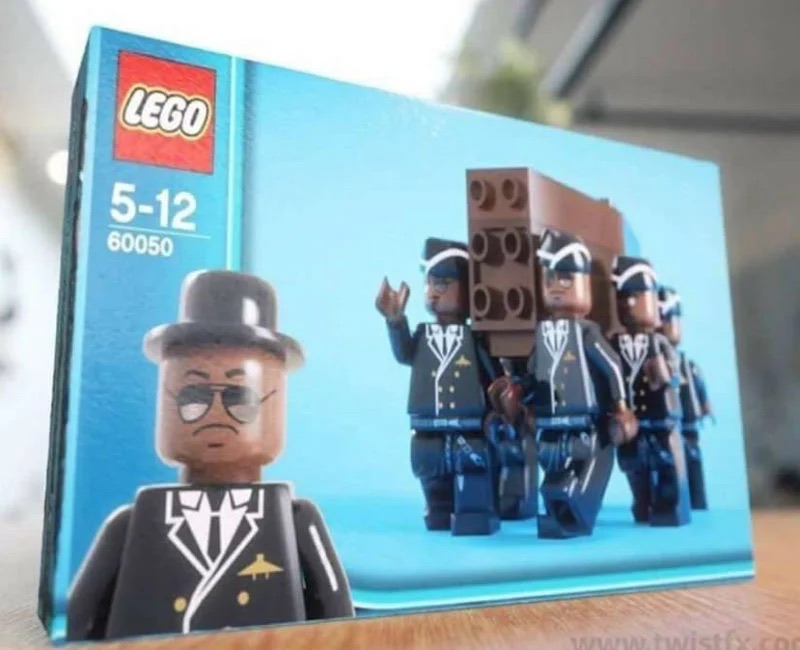
\includegraphics[width=10cm]{Bilddateien/CoffinDance.jpg}
%    \label{fig:myfreshbild}
%\end{figure}

In this experiment, the nuclear magnetic resonance (NMR) is studied in a simple water probe. Firstly, parameters for a clear resonance signal are investigated. Using this signal, the relaxation times for spin-lattice- and spin-spin-relaxtion are measured. In the process of this, typical NMR-pulse sequences are familiarized: namley, the spin-echo and Carr-Purcell-Meiboom-Gill (CPMG) sequence. Furthermore the im\\

An important application of NMR is in MRI

\end{document}